\documentclass[a4paper,11pt,twoside]{scrartcl}
\usepackage[T1]{fontenc}
\usepackage{subcaption}
\usepackage[utf8]{inputenc}
\usepackage{ngerman, eucal, mathrsfs, amsfonts, bbm, amsmath, amssymb, stmaryrd,graphicx, array, geometry, color, wrapfig, float, hyperref, epstopdf,gensymb, subcaption, extarrows}
\usepackage[controls, step, poster=first]{animate}
\geometry{left=25mm, right=15mm, bottom=25mm}
\setlength{\parindent}{0em} 
\setlength{\headheight}{0em} 
\title{Graphenalgorithmen\\ Blatt 8}
\author{Markus Vieth\and Christian Stricker}
\date{\today}
\input{../head/lstlisting.tex}
\usepackage{float}
\usepackage[section]{placeins}
\usepackage{epstopdf}
\usepackage{wrapfig}
\usepackage{caption}
\usepackage{subcaption}
\usepackage{graphicx}
\usepackage{pgfplots}
\usepackage[usenames,dvipsnames,svgnames,table]{xcolor}
\usetikzlibrary{plotmarks}
\usetikzlibrary{patterns}
\usetikzlibrary{decorations.pathmorphing}
\usetikzlibrary{calc}
\usetikzlibrary{shapes}
\newcommand{\coloredcircled}[3][black]{{\large \Large\color{#2}\textcircled {{\small\color{#1}#3}}}}% Circlecolor, Textcolor, text
\newcommand{\ddvec}[2]{\begin{pmatrix}#1\\#2\end{pmatrix}}
\newcommand{\dddvec}[3]{\begin{pmatrix}#1\\#2\\#3\end{pmatrix}}
\newcommand{\longvec}[1]{\overset{\longrightarrow}{#1}}
\newcommand{\eunorm}[1]{\left\lVert#1\right\rVert_2}
\newcommand{\scalar}[2]{\left<#1,#2\right>}\newcommand{\cor}[1]{\textcolor{red}{\textit{#1}}}
\newcommand{\qed}{%
	\begin{flushright}
		q.e.d.
	\end{flushright}%
	}
\begin{document}
\maketitle
\cleardoublepage
\pagestyle{myheadings}
\markboth{Markus Vieth, Christian Stricker}{Markus Vieth, Christian Stricker}

\newpage
\section{Aufgabe 1: Separator im Graphen $G$ (10 Punkte)}
\section{Aufgabe 2: Cops and Robber (10 Punkte)}
\section{Aufgabe 3: Baumzerlegung berechnen (20 Punkte)}
\subsection{a}
\begin{animateinline}{2}
\begin{figure}[H]
	\centering
	\begin{subfigure}{.33\textwidth}
		\centering
		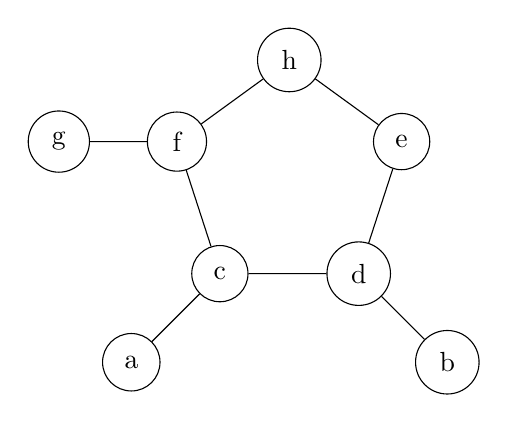
\begin{tikzpicture}[scale=1.5, every node/.style={draw,circle, align=center, inner sep = .5em}]
		\node at (90:1) (h) {h};
		\node at (90-72:1) (e) {e};
		\node at (90-72*2:1) (d) {d};
		\node at (90-72*3:1) (c) {c};
		\node at (90-72*4:1) (f) {f};
		\node at ($(f) + (-1,0)$) (g) {g};
		\node at ($ (c) - (.75,.75) $) (a) {a};
		\node at ($ (d) + (.75,-.75) $) (b) {b};
		\draw (g) -- (f) -- (h) -- (e) -- (d) -- (c) -- (f) (a) -- (c) (b) -- (d);
		\end{tikzpicture}
		\caption{Graph $G$}
	\end{subfigure}
	\begin{subfigure}{.66\textwidth}
		\centering
		\begin{tikzpicture}[scale=2, every node/.style={draw,circle, align=center, inner sep = .5em}]
		\node[rectangle] at (-2,2.5)   {$U = \emptyset$};
		\node[rectangle] at (-2,2)   {$C = \{a,b,c,d,e,f,g\}$};
		\node[rectangle] at (-2,1.5) {$X = \emptyset$};
		\node[rectangle] at (-2,1.0)   {$t = /$};
		\node[rectangle] at (-2,.5)  {$C \ni n_c  = c$};
		
		\node[ellipse, label =0:$X_1$] {$c$};
		
		\end{tikzpicture}
		\caption{Tree decomposition $T$}
		\end{subfigure}
		\caption{Ausgangssituation}
\end{figure}
\newframe
\begin{figure}[H]
	\centering
	\begin{subfigure}{.33\textwidth}
		\centering
		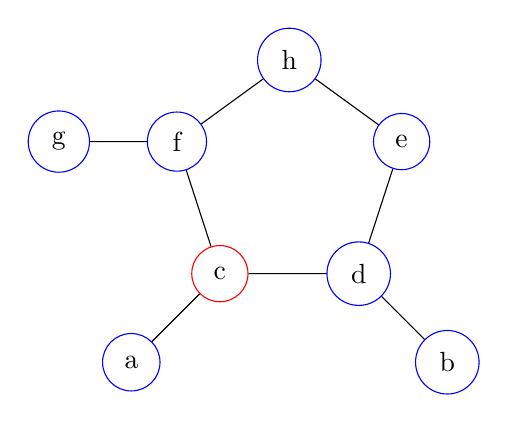
\begin{tikzpicture}[scale=1.5, every node/.style={draw=blue,circle, align=center, inner sep = .5em}]
		\node at (90:1) (h) {h};
		\node at (90-72:1) (e) {e};
		\node at (90-72*2:1) (d) {d};
		\node[draw=red] at (90-72*3:1) (c) {c};
		\node at (90-72*4:1) (f) {f};
		\node at ($(f) + (-1,0)$) (g) {g};
		\node at ($ (c) - (.75,.75) $) (a) {a};
		\node at ($ (d) + (.75,-.75) $) (b) {b};
		\draw (g) -- (f) -- (h) -- (e) -- (d) -- (c) -- (f) (a) -- (c) (b) -- (d);
		\end{tikzpicture}
		\caption{\color{blue}$V\setminus U$ | \color{red} $U$}
	\end{subfigure}
	\begin{subfigure}{.66\textwidth}
		\centering
		\begin{tikzpicture}[sibling distance = 10em, level distance = 1.5em, scale=2, every node/.style={draw, ellipse, align=center, inner sep = .5em}]
		\node[rectangle] at (-2,2.5)   {$U = \{c\}$};
		\node[rectangle] at (-2,2)   {$C = \{a\}$};
		\node[rectangle] at (-2,1.5) {$X = \{c\}$};
		\node[rectangle] at (-2,1.0) {$t = 1$};
		\node[rectangle] at (-2,.5)  {$C \ni n_c  = a$};
		
		\node[label =0:$X_1$] at (0,3){$c$}
		child{
			node[label=0:$X_2$] {$a,c$}	
		};
		\end{tikzpicture}
		\caption{Tree decomposition $T$}
	\end{subfigure}
\end{figure}
\newframe
\begin{figure}[H]
	\centering
	\begin{subfigure}{.33\textwidth}
		\centering
		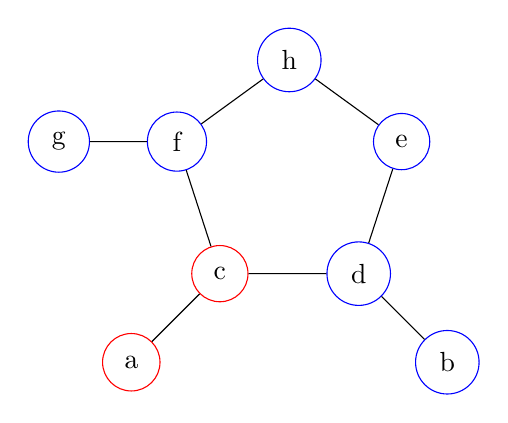
\begin{tikzpicture}[scale=1.5, every node/.style={draw=blue,circle, align=center, inner sep = .5em}]
		\node at (90:1) (h) {h};
		\node at (90-72:1) (e) {e};
		\node at (90-72*2:1) (d) {d};
		\node[draw=red] at (90-72*3:1) (c) {c};
		\node at (90-72*4:1) (f) {f};
		\node at ($(f) + (-1,0)$) (g) {g};
		\node[draw=red] at ($ (c) - (.75,.75) $) (a) {a};
		\node at ($ (d) + (.75,-.75) $) (b) {b};
		\draw (g) -- (f) -- (h) -- (e) -- (d) -- (c) -- (f) (a) -- (c) (b) -- (d);
		\end{tikzpicture}
		\caption{\color{blue}$V\setminus U$ | \color{red} $U$}
	\end{subfigure}
	\begin{subfigure}{.66\textwidth}
		\centering
		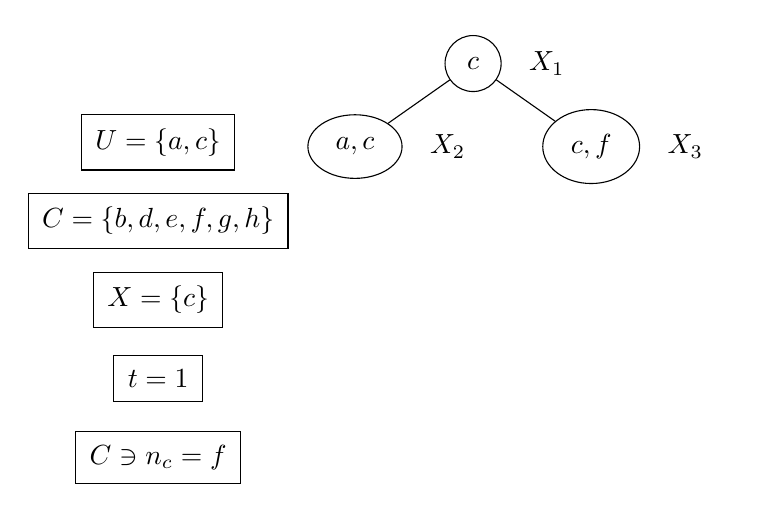
\begin{tikzpicture}[level distance = 1.5em, scale=2, every node/.style={draw, ellipse, align=center, inner sep = .5em}]
		\node[rectangle] at (-2,2.5)   {$U = \{a, c\}$};
		\node[rectangle] at (-2,2)   {$C = \{b,d,e,f,g,h\}$};
		\node[rectangle] at (-2,1.5) {$X = \{c\}$};
		\node[rectangle] at (-2,1.0) {$t = 1$};
		\node[rectangle] at (-2,.5)  {$ C \ni n_c = f$};
		
		\node[label =0:$X_1$] at (0,3){$c$}
		child{
			node[label=0:$X_2$] {$a,c$}	
		}
		child{
			node[label=0:$X_3$] {$c,f$}
		};
		\end{tikzpicture}
		\caption{Tree decomposition $T$}
	\end{subfigure}
\end{figure}
\newframe
\begin{figure}[H]
	\centering
	\begin{subfigure}{.33\textwidth}
		\centering
		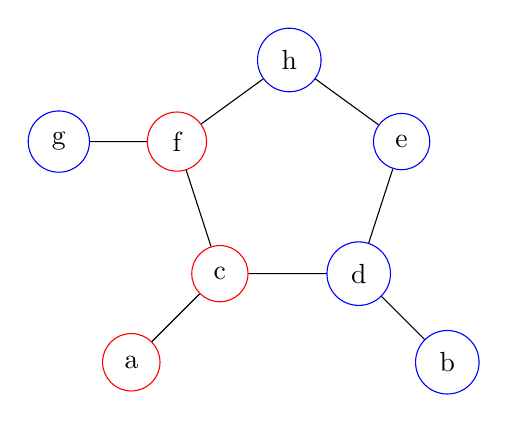
\begin{tikzpicture}[scale=1.5, every node/.style={draw=blue,circle, align=center, inner sep = .5em}]
		\node at (90:1) (h) {h};
		\node at (90-72:1) (e) {e};
		\node at (90-72*2:1) (d) {d};
		\node[draw=red] at (90-72*3:1) (c) {c};
		\node[draw=red] at (90-72*4:1) (f) {f};
		\node at ($(f) + (-1,0)$) (g) {g};
		\node[draw=red] at ($ (c) - (.75,.75) $) (a) {a};
		\node at ($ (d) + (.75,-.75) $) (b) {b};
		\draw (g) -- (f) -- (h) -- (e) -- (d) -- (c) -- (f) (a) -- (c) (b) -- (d);
		\end{tikzpicture}
		\caption{\color{blue}$V\setminus U$ | \color{red} $U$}
	\end{subfigure}
	\begin{subfigure}{.66\textwidth}
		\centering
		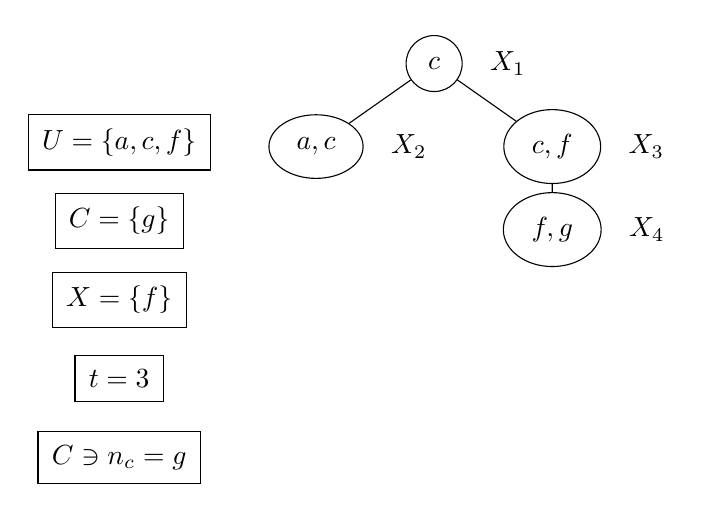
\begin{tikzpicture}[level distance = 1.5em, scale=2, every node/.style={draw, ellipse, align=center, inner sep = .5em}]
		\node[rectangle] at (-2,2.5)   {$U = \{a,c,f\}$};
		\node[rectangle] at (-2,2)   {$C = \{g\}$};
		\node[rectangle] at (-2,1.5) {$X = \{f\}$};
		\node[rectangle] at (-2,1.0) {$t = 3$};
		\node[rectangle] at (-2,.5)  {$ C \ni n_c = g$};
		
		
		\node[label =0:$X_1$] at (0,3){$c$}
		child{
			node[label=0:$X_2$] {$a,c$}	
		}
		child{
			node[label=0:$X_3$] {$c,f$}
			child{
				node[label=0:$X_4$] {$f,g$}	
			}
		};
		
		\end{tikzpicture}
		\caption{Tree decomposition $T$}
	\end{subfigure}
\end{figure}
\newframe
\begin{figure}[H]
	\centering
	\begin{subfigure}{.33\textwidth}
		\centering
		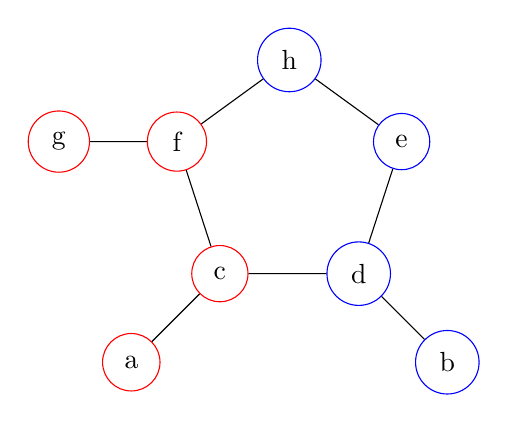
\begin{tikzpicture}[scale=1.5, every node/.style={draw=blue,circle, align=center, inner sep = .5em}]
		\node at (90:1) (h) {h};
		\node at (90-72:1) (e) {e};
		\node at (90-72*2:1) (d) {d};
		\node[draw=red] at (90-72*3:1) (c) {c};
		\node[draw=red] at (90-72*4:1) (f) {f};
		\node[draw=red] at ($(f) + (-1,0)$) (g) {g};
		\node[draw=red] at ($ (c) - (.75,.75) $) (a) {a};
		\node at ($ (d) + (.75,-.75) $) (b) {b};
		\draw (g) -- (f) -- (h) -- (e) -- (d) -- (c) -- (f) (a) -- (c) (b) -- (d);
		\end{tikzpicture}
		\caption{\color{blue}$V\setminus U$ | \color{red} $U$}
	\end{subfigure}
	\begin{subfigure}{.66\textwidth}
		\centering
		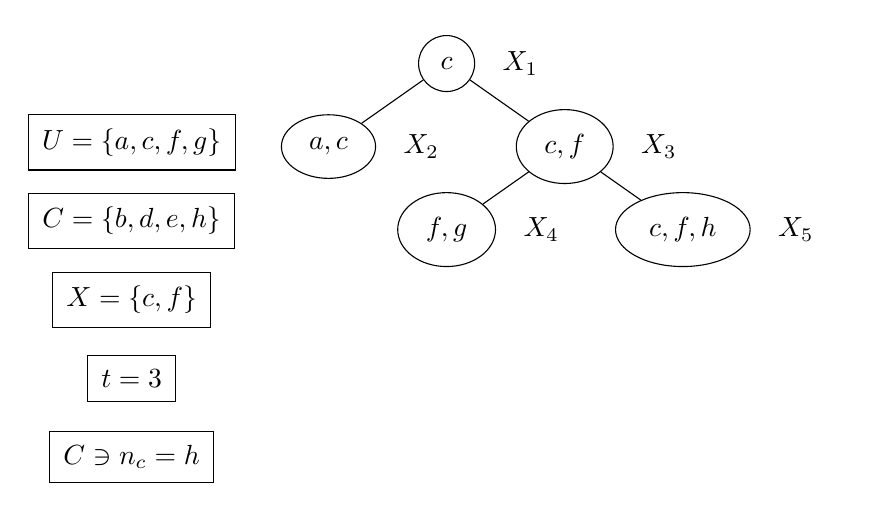
\begin{tikzpicture}[level distance = 1.5em, scale=2, every node/.style={draw, ellipse, align=center, inner sep = .5em}]
		\node[rectangle] at (-2,2.5)   {$U = \{a,c,f,g\}$};
		\node[rectangle] at (-2,2)   {$C = \{b,d,e,h\}$};
		\node[rectangle] at (-2,1.5) {$X = \{c, f\}$};
		\node[rectangle] at (-2,1.0) {$t = 3$};
		\node[rectangle] at (-2,.5)  {$ C \ni n_c = h$};
		
		
		\node[label =0:$X_1$] at (0,3){$c$}
		child{
			node[label=0:$X_2$] {$a,c$}	
		}
		child{
			node[label=0:$X_3$] {$c,f$}
			child{
				node[label=0:$X_4$] {$f,g$}	
			}
			child{
				node[label=0:$X_5$] {$c,f,h$}	
			}
		};
		
		\end{tikzpicture}
		\caption{Tree decomposition $T$}
	\end{subfigure}
\end{figure}
\newframe
\begin{figure}[H]
	\centering
	\begin{subfigure}{.33\textwidth}
		\centering
		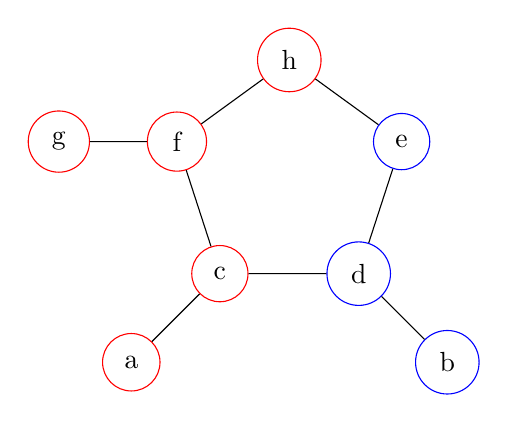
\begin{tikzpicture}[scale=1.5, every node/.style={draw=blue,circle, align=center, inner sep = .5em}]
		\node[draw=red] at (90:1) (h) {h};
		\node at (90-72:1) (e) {e};
		\node at (90-72*2:1) (d) {d};
		\node[draw=red] at (90-72*3:1) (c) {c};
		\node[draw=red] at (90-72*4:1) (f) {f};
		\node[draw=red] at ($(f) + (-1,0)$) (g) {g};
		\node[draw=red] at ($ (c) - (.75,.75) $) (a) {a};
		\node at ($ (d) + (.75,-.75) $) (b) {b};
		\draw (g) -- (f) -- (h) -- (e) -- (d) -- (c) -- (f) (a) -- (c) (b) -- (d);
		\end{tikzpicture}
		\caption{\color{blue}$V\setminus U$ | \color{red} $U$}
	\end{subfigure}
	\begin{subfigure}{.66\textwidth}
		\centering
		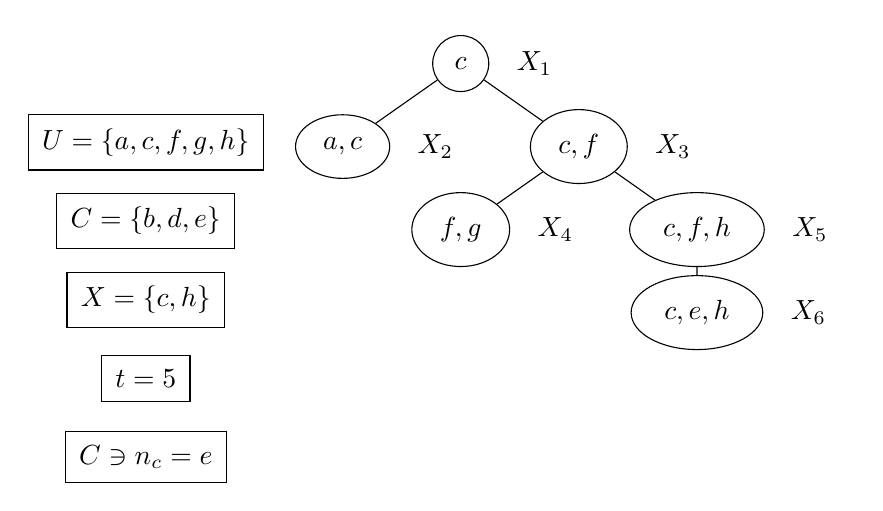
\begin{tikzpicture}[level distance = 1.5em, scale=2, every node/.style={draw, ellipse, align=center, inner sep = .5em}]
		\node[rectangle] at (-2,2.5)   {$U = \{a,c,f,g,h\}$};
		\node[rectangle] at (-2,2)   {$C = \{b,d,e\}$};
		\node[rectangle] at (-2,1.5) {$X = \{c, h\}$};
		\node[rectangle] at (-2,1.0) {$t = 5$};
		\node[rectangle] at (-2,.5)  {$ C \ni n_c = e$};
		
		
		\node[label =0:$X_1$] at (0,3){$c$}
		child{
			node[label=0:$X_2$] {$a,c$}	
		}
		child{
			node[label=0:$X_3$] {$c,f$}
			child{
				node[label=0:$X_4$] {$f,g$}	
			}
			child{
				node[label=0:$X_5$] {$c,f,h$}	
				child {
					node[label=0:$X_6$] {$c,e,h$}	
				}
			}
		};
		
		\end{tikzpicture}
		\caption{Tree decomposition $T$}
	\end{subfigure}
\end{figure}
\newframe
\begin{figure}[H]
	\centering
	\begin{subfigure}{.33\textwidth}
		\centering
		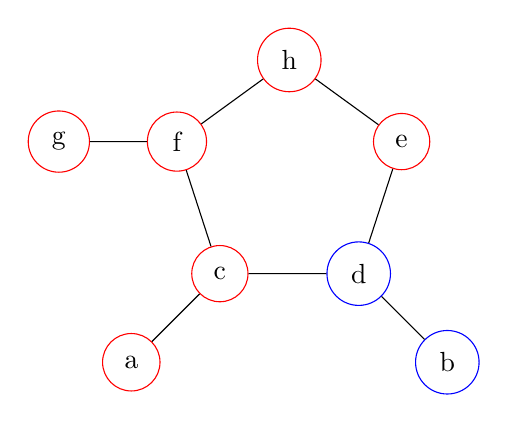
\begin{tikzpicture}[scale=1.5, every node/.style={draw=blue,circle, align=center, inner sep = .5em}]
		\node[draw=red] at (90:1) (h) {h};
		\node[draw=red] at (90-72:1) (e) {e};
		\node at (90-72*2:1) (d) {d};
		\node[draw=red] at (90-72*3:1) (c) {c};
		\node[draw=red] at (90-72*4:1) (f) {f};
		\node[draw=red] at ($(f) + (-1,0)$) (g) {g};
		\node[draw=red] at ($ (c) - (.75,.75) $) (a) {a};
		\node at ($ (d) + (.75,-.75) $) (b) {b};
		\draw (g) -- (f) -- (h) -- (e) -- (d) -- (c) -- (f) (a) -- (c) (b) -- (d);
		\end{tikzpicture}
		\caption{\color{blue}$V\setminus U$ | \color{red} $U$}
	\end{subfigure}
	\begin{subfigure}{.66\textwidth}
		\centering
		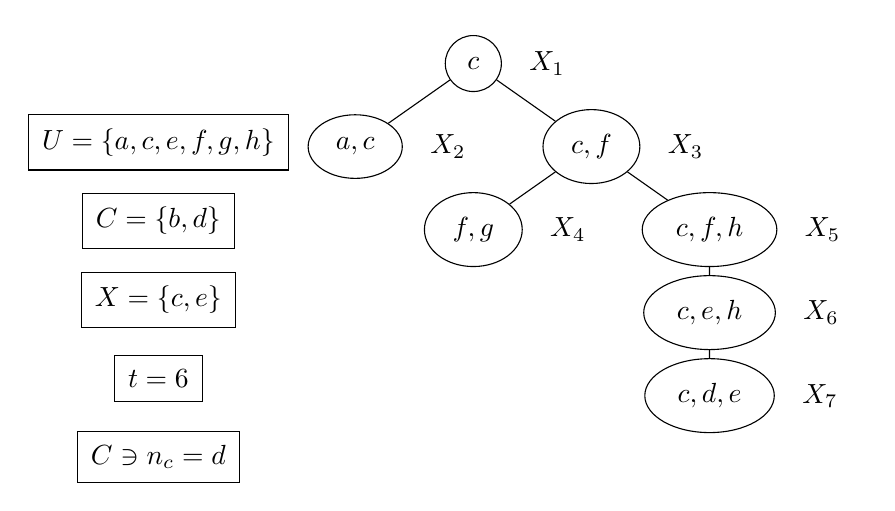
\begin{tikzpicture}[level distance = 1.5em, scale=2, every node/.style={draw, ellipse, align=center, inner sep = .5em}]
		\node[rectangle] at (-2,2.5)   {$U = \{a,c,e,f,g,h\}$};
		\node[rectangle] at (-2,2)   {$C = \{b,d\}$};
		\node[rectangle] at (-2,1.5) {$X = \{c, e\}$};
		\node[rectangle] at (-2,1.0) {$t = 6$};
		\node[rectangle] at (-2,.5)  {$ C \ni n_c = d$};
		
		
		\node[label =0:$X_1$] at (0,3){$c$}
		child{
			node[label=0:$X_2$] {$a,c$}	
		}
		child{
			node[label=0:$X_3$] {$c,f$}
			child{
				node[label=0:$X_4$] {$f,g$}	
			}
			child{
				node[label=0:$X_5$] {$c,f,h$}	
				child {
					node[label=0:$X_6$] {$c,e,h$}
					child{
						node[label=0:$X_7$] {$c,d,e$}	
					}	
				}
			}
		};
		
		\end{tikzpicture}
		\caption{Tree decomposition $T$}
	\end{subfigure}
\end{figure}
\newframe
\begin{figure}[H]
	\centering
	\begin{subfigure}{.33\textwidth}
		\centering
		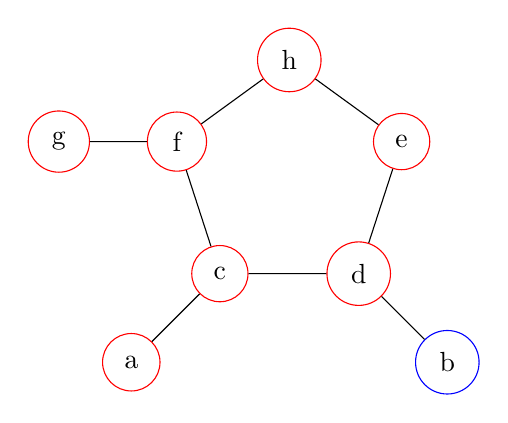
\begin{tikzpicture}[scale=1.5, every node/.style={draw=blue,circle, align=center, inner sep = .5em}]
		\node[draw=red] at (90:1) (h) {h};
		\node[draw=red] at (90-72:1) (e) {e};
		\node[draw=red] at (90-72*2:1) (d) {d};
		\node[draw=red] at (90-72*3:1) (c) {c};
		\node[draw=red] at (90-72*4:1) (f) {f};
		\node[draw=red] at ($(f) + (-1,0)$) (g) {g};
		\node[draw=red] at ($ (c) - (.75,.75) $) (a) {a};
		\node at ($ (d) + (.75,-.75) $) (b) {b};
		\draw (g) -- (f) -- (h) -- (e) -- (d) -- (c) -- (f) (a) -- (c) (b) -- (d);
		\end{tikzpicture}
		\caption{\color{blue}$V\setminus U$ | \color{red} $U$}
	\end{subfigure}
	\begin{subfigure}{.66\textwidth}
		\centering
		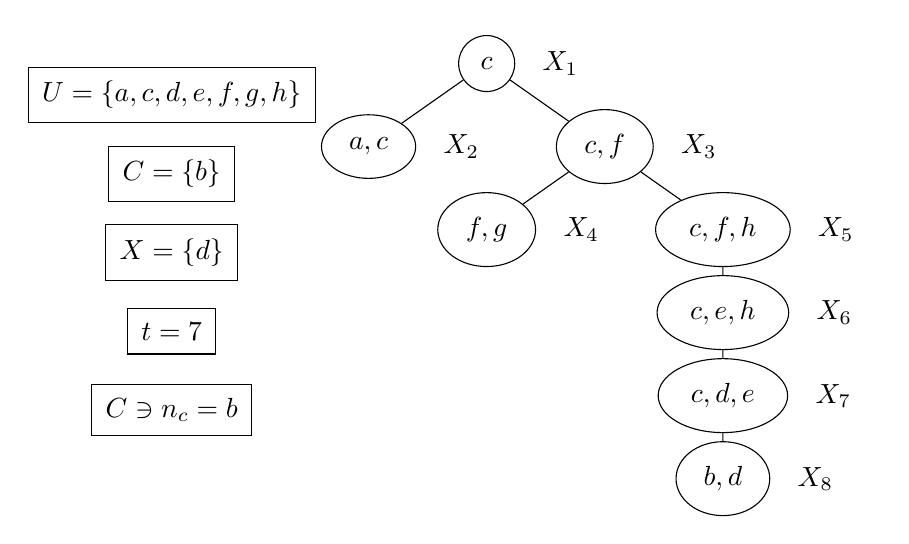
\begin{tikzpicture}[level distance = 1.5em, scale=2, every node/.style={draw, ellipse, align=center, inner sep = .5em}]
		\node[rectangle] at (-2,2.5)   {$U = \{a,c,d,e,f,g,h\}$};
		\node[rectangle] at (-2,2)   {$C = \{b\}$};
		\node[rectangle] at (-2,1.5) {$X = \{d\}$};
		\node[rectangle] at (-2,1.0) {$t = 7$};
		\node[rectangle] at (-2,.5)  {$ C \ni n_c = b$};
		
		
		\node[label =0:$X_1$] at (0,2.7){$c$}
		child{
			node[label=0:$X_2$] {$a,c$}	
		}
		child{
			node[label=0:$X_3$] {$c,f$}
			child{
				node[label=0:$X_4$] {$f,g$}	
			}
			child{
				node[label=0:$X_5$] {$c,f,h$}	
				child {
					node[label=0:$X_6$] {$c,e,h$}
					child{
						node[label=0:$X_7$] {$c,d,e$}
						child{
							node[label=0:$X_8$] {$b,d$}	
						}
					}	
				}
			}
		};
		
		\end{tikzpicture}
		\caption{Tree decomposition $T$}
	\end{subfigure}
\end{figure}
\end{animateinline}
\begin{figure}[H]
	\centering
	\begin{subfigure}{.45\textwidth}
		\centering
		\begin{tikzpicture}[scale=2, every node/.style={draw,circle, align=center, inner sep = .5em}]
		\node at (90:1) (h) {h};
		\node at (90-72:1) (e) {e};
		\node at (90-72*2:1) (d) {d};
		\node at (90-72*3:1) (c) {c};
		\node at (90-72*4:1) (f) {f};
		\node at ($(f) + (-1,0)$) (g) {g};
		\node at ($ (c) - (.75,.75) $) (a) {a};
		\node at ($ (d) + (.75,-.75) $) (b) {b};
		\draw (g) -- (f) -- (h) -- (e) -- (d) -- (c) -- (f) (a) -- (c) (b) -- (d);
		\end{tikzpicture}
		\caption{Graph $G$}
	\end{subfigure}
	\begin{subfigure}{.45\textwidth}
		\centering
		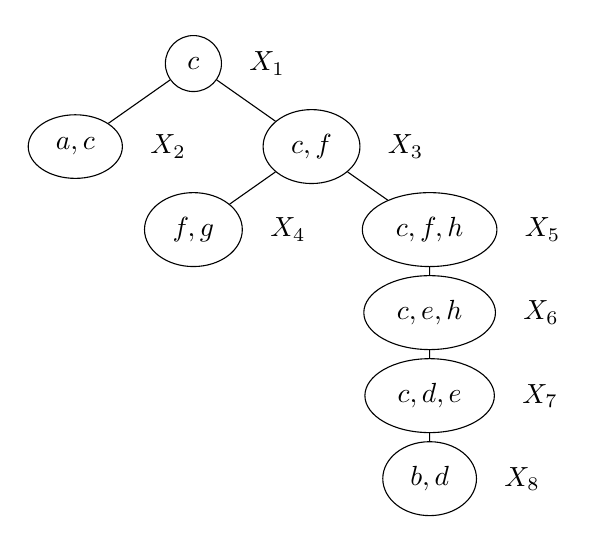
\begin{tikzpicture}[level distance = 1.5em, scale=2, every node/.style={draw, ellipse, align=center, inner sep = .5em}]
		\node[label =0:$X_1$] {$c$}
		child{
			node[label=0:$X_2$] {$a,c$}	
		}
		child{
			node[label=0:$X_3$] {$c,f$}
			child{
				node[label=0:$X_4$] {$f,g$}	
			}
			child{
				node[label=0:$X_5$] {$c,f,h$}	
				child {
					node[label=0:$X_6$] {$c,e,h$}
					child{
						node[label=0:$X_7$] {$c,d,e$}
						child{
							node[label=0:$X_8$] {$b,d$}	
						}
					}	
				}
			}
		};
		
		\end{tikzpicture}
		\caption{Tree decomposition $T$}
	\end{subfigure}
	\caption{Result}
\end{figure}

\end{document}